\documentclass[tikz,border=0pt,convert={density=1000,size=2000x1000,outext=.png}]{standalone}
\usepackage{tikz}

\usetikzlibrary{backgrounds,arrows,shapes,shapes.misc,shapes.arrows,chains,matrix,positioning,scopes,decorations.pathmorphing,shadows}

\tikzset{
	state/.style={
		rectangle,
		rounded corners,
		draw=black, very thick,
		minimum height=2em,
		inner sep=2pt,
		text centered,
	},
}

\usepackage{amsmath,amssymb}

\usepackage{color}

\definecolor{light-gray}{gray}{0.9}
\begin{document}

\begin{footnotesize}

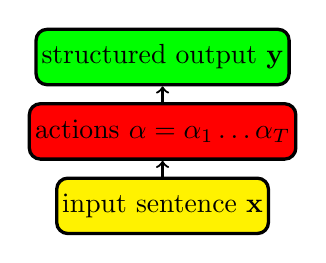
\begin{tikzpicture}[node distance=2mm]
\node	(input)	[state, fill=yellow]			{input sentence $\mathbf{x}$};
\node	(actions)				[state, fill=red]	[above=of input]	{actions $\mathbf{\alpha}=\alpha_1\ldots\alpha_T$};
\node	(output)				[state, fill=green]	[above=of actions]	{structured output $\mathbf{y}$};

%\node	(theme)	[component]		[below=of trigger]	{theme assignment};
%\node	(theme_in)	[input]		[left=of theme]		{themes};
%\node	(cause)	[component]		[below=of theme]	{cause assignment};
%\node	(cause_in)	[input]		[left=of cause]		 {causes};
%\path[thick, ->] (trigger_in) edge (trigger);
\path[thick, ->] (actions) edge (output);
\path[thick, ->] (input) edge (actions);

\end{tikzpicture}

	
\end{footnotesize}

\end{document}